%%%%%%%%%%%%%%%%%%%%%%%%%%%%%%%%%%%%%%%%%%%%%%%%%%%%%%%%%
\documentclass{elsarticle}
				
\usepackage[a4paper]{geometry} % change page margins
\usepackage[utf8]{inputenc}
\usepackage{amsmath}
%\usepackage{amssymb}
\usepackage{empheq}
\usepackage{bm} % bold math
%\usepackage{chemfig}

\usepackage{stix}

\usepackage{graphicx}
\usepackage{epstopdf} 
%\epstopdfsetup{outdir=./}
\usepackage{multirow}
\usepackage{tocbasic}
%\usepackage{subfig}
\usepackage{caption}
\usepackage{subcaption}
\usepackage{placeins}%for float barrier
%\usepackage[shortcuts]{extdash}
\usepackage{siunitx}
%\usepackage{mdframed}
%\usepackage{url}
%\usepackage{framed}
%\usepackage{lscape} % landscape pages
\usepackage{booktabs} % professional tables
\usepackage{color}
%\usepackage{todonotes} % todo's
%\usepackage{cleveref} % clever references using \cref
%\usepackage{empheq}

\graphicspath{{figures/}}
\usepackage{hyperref} % references become links

\setcounter{secnumdepth}{3}
\setcounter{tocdepth}{3}

\newcommand{\vt}[1]{\bm{#1}}
\newcommand{\rd}{\textrm{d}}
\newcommand{\Rey}{\textrm{Re}}
\newcommand{\wt}[1]{\left\langle #1 \right\rangle}
\newcommand{\wh}[1]{\left\lbrace #1 \right\rbrace}
\newcommand{\dd}[2]{\frac{\partial #1}{\partial #2}}
\newcommand{\ul}[1]{\underline{#1}} 
\newcommand{\md}{\mathrm{d}}
\newcommand{\degree}{^{\circ}}

\newcommand{\hl}[1]{\textcolor{black}{#1}}
\newcommand{\hll}[1]{\textcolor{blue}{#1}}

\makeatletter
\def\ps@pprintTitle{%
 \let\@oddhead\@empty
 \let\@evenhead\@empty
 \def\@oddfoot{}%
 \let\@evenfoot\@oddfoot}
\makeatother

%\usepackage{helvet}
%\usepackage{lmodern}
%\fontfamily{lmss}\selectfont

\listfiles

\begin{document}

\title{Sensitivity analysis with stochastic models}              % mandatory field
\author[add1]{B. Sanderse}
\ead{B.Sanderse@cwi.nl, corresponding author}
%\author[add1,add3]{J.F.H. Buist}
%\author[add2,add3]{R.A.W.M. Henkes}

\address[add1]{Centrum Wiskunde \& Informatica (CWI), Amsterdam, The Netherlands}
%\address[add2]{Shell Technology Centre Amsterdam, Amsterdam, The Netherlands}
%\address[add3]{Delft University of Technology, Delft, The Netherlands}



\begin{abstract}
Abstract
\end{abstract}

\begin{keyword}
Stochastic model, sensitivity analysis
\end{keyword}

%\date{\today}

\maketitle  


%\tableofcontents

%%%%%%%%%%%%%%%%%%%%%%%%%%%%%%%%%%%%%%%%%%%%%%%%%%%%%%%%%
%%%%%%%%%%%%%%%%%      Main matter     %%%%%%%%%%%%%%%%%%
%%%%%%%%%%%%%%%%%%%%%%%%%%%%%%%%%%%%%%%%%%%%%%%%%%%%%%%%%
\section{Introduction}
Consider the following model (inspired by \cite{Zhu2020a}):
\begin{equation}\label{eqn:example}
Y(\vt{x},\omega) = \sin(x_{1}) + 7 \sin(x_{2})^2 + \exp( Z_{1} + (x_{1}/\pi) Z_{2}(\omega)),
\end{equation}
where $\vt{x}$ denotes the input parameters $X_{1},X_{2} \sim \mathcal{U}(0,2\pi)$, and $Z$ denotes the latent variables that introduce `internal' stochasticity into the model, $Z_{1} \sim \mathcal{U}(0,1)$, $Z_{2} \sim \mathcal{N}(0,1)$.
The effect of $Z$ on $Y$ can be present in different ways, depending on how much is known about $Z$:
\begin{enumerate}
\item Treat $Z$ as an additional parameter making the model deterministic:
\begin{equation}
Y(\hat{\vt{x}}) = \sin(x_{1}) + 7 \sin(x_{2})^2 + \exp( x_{3} + (x_{1}/\pi) x_{4}),
\end{equation}
with $X_{3}\sim \mathcal{U}(0,1)$ and $X_{4}\sim \mathcal{N}(0,1)$. This requires explicit knowledge of the internal stochasticity, i.e.\ the expression for $Z$. The input space is now four-dimensional. In this case one can use existing UQ techniques, such as polynomial chaos expansions.
\item Treat $Z$ via the random seed. This is a slightly less intrusive approach only requiring access to the random seed. We take $X_{3} \sim \mathcal{U}(2^{14}, 2^{16})$ (rounded to give integer values), which sets the value for the random seed: $\texttt{seed}(X_{3})$, and then $Z_{1} \sim \mathcal{U}(0,1)$, $Z_{2} \sim \mathcal{N}(0,1)$. In this case the input space is three-dimensional instead of four-dimensional.
\item Don't treat $Z$: in case no access is given to $Z$ (a black-box code in which only $X$ can be controlled), and the actual form \eqref{eqn:example} is not known, one can only sample a two-dimensional parameter space ($X_{1}$, $X_{2}$), and has to depend on the stochasticity introduced by the black-box code.
\end{enumerate}

Depending on the type of access to the latent variables $Z$, different approaches are possible to perform a global sensitivity analysis (Sobol' analysis):
\begin{itemize}
\item Classic analysis: extend $\vt{X}$ with the latent variables $Z$, turning the stochastic simulator in a deterministic one. This requires type 1 or type 2 access.
\item QoI-based analysis: define a statistical quantity (called the quantity of interest in \cite{Zhu2020a}) which eliminates the randomness due to $Z$. For example, take the mean $m(\vt{x})$ (expectation over $Z$), and then the sensitivity analysis is performed for the mean instead of for the output $Y$. In other words, one first integrates over $Z$ to get a deterministic quantity, and then integrates over $X$ for the Sobol' analysis.
\item Trajectory-based analysis. In this case the steps of the QoI-based analysis are reversed. In this case one first fixes a value for $Z$, does the Sobol' analysis with respect to $X$, and then repeats for different values of $Z$ and takes the expectation.
\end{itemize}


\section{Example results}
Classical analysis with type 1 access is shown in figure \ref{fig:type1}, based on Monte Carlo simulation. We set $M=10^{4}$ samples, but in reality $N =12 M$ samples are needed to compute the first and second order indices. The total and first order indices require $M (p+2) = 6 M$ ($p=4$) evaluations (Saltelli method), and the second order indices require $M \cdot {p \choose 2} = 6 M$ evaluations.

\begin{figure}[hbtp]
\centering
	\begin{subfigure}[b]{.49\textwidth}
	\centering
	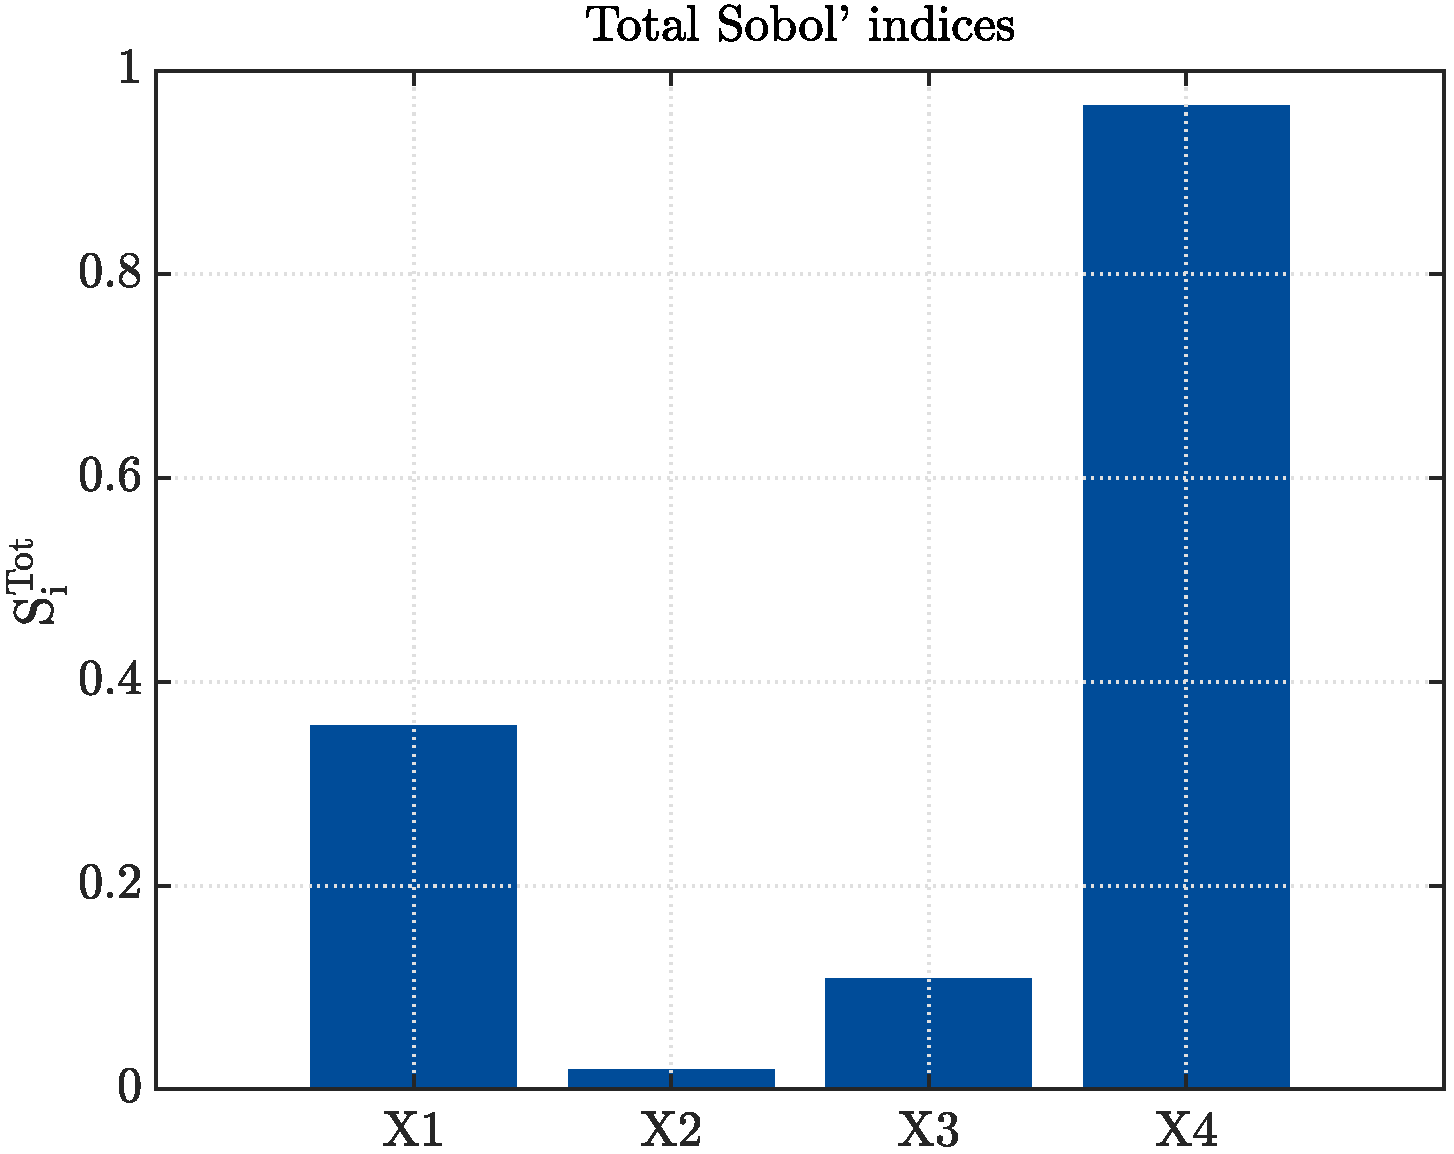
\includegraphics[width=\textwidth]{figures/total_type1.pdf}
	\caption{Total index.\label{fig:total_type1}}
	\end{subfigure}
	\hfill
	\begin{subfigure}[b]{.49\textwidth}
	\centering
	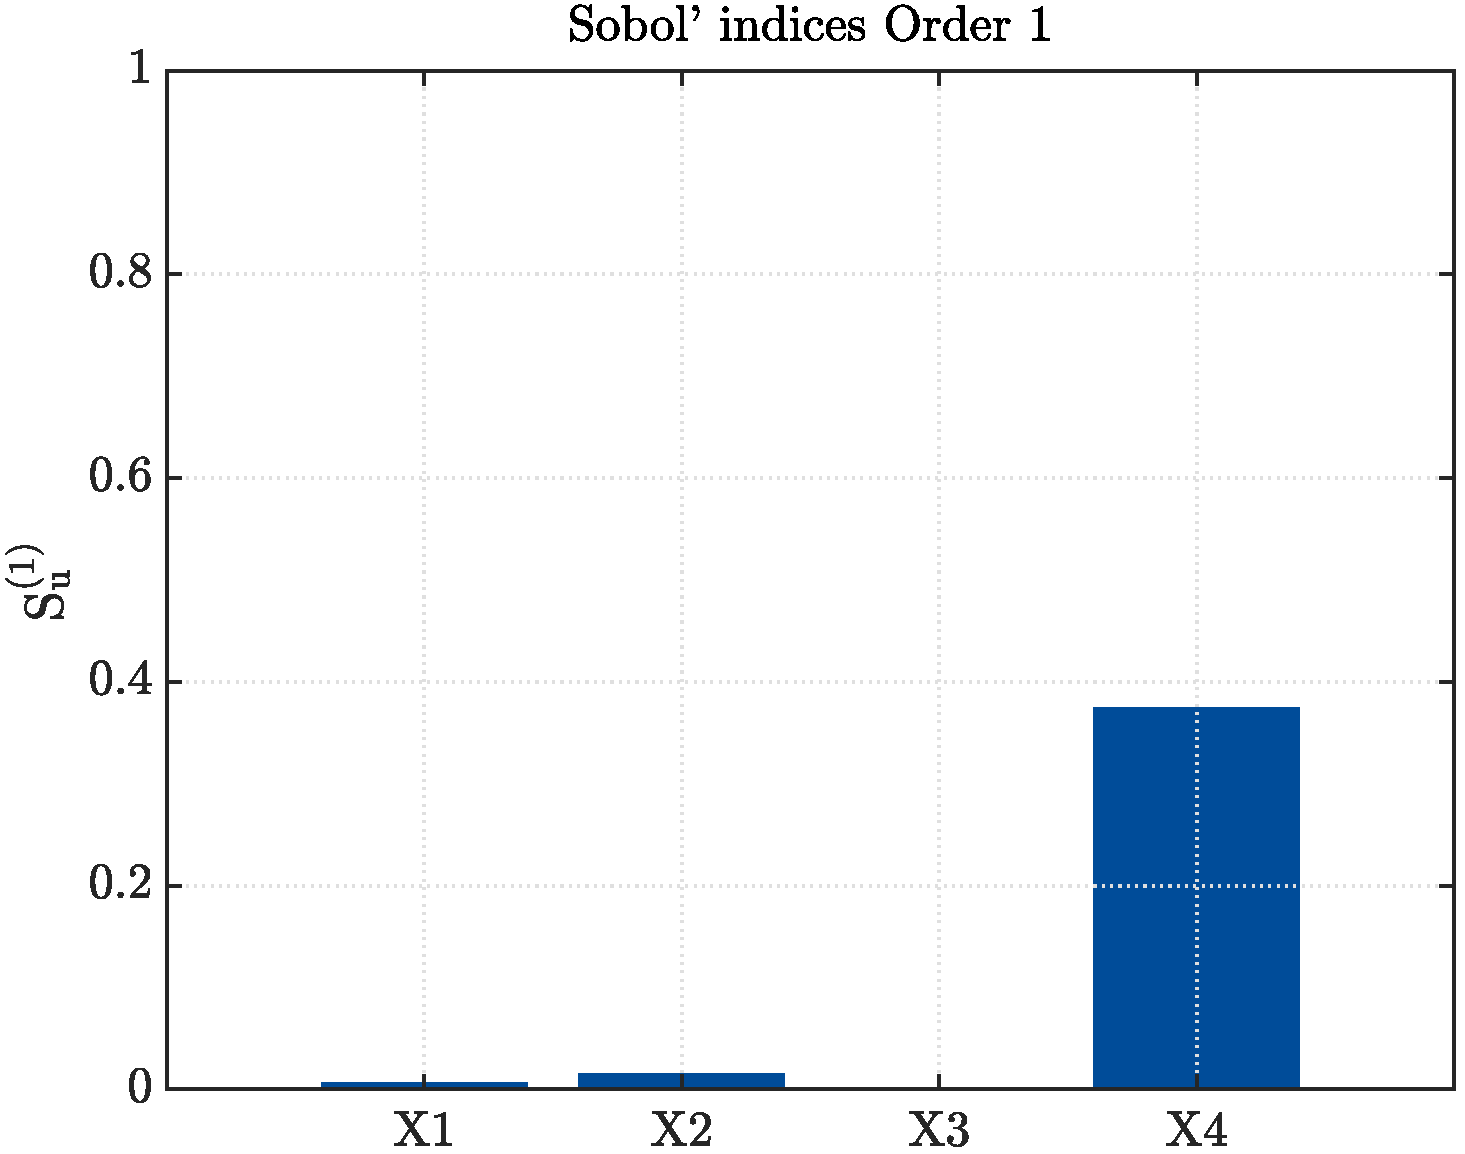
\includegraphics[width=\textwidth]{figures/first_type1.pdf}
	\caption{First order.\label{fig:first_type1}}
	\end{subfigure}\\
	\begin{subfigure}[b]{.49\textwidth}
	\centering
	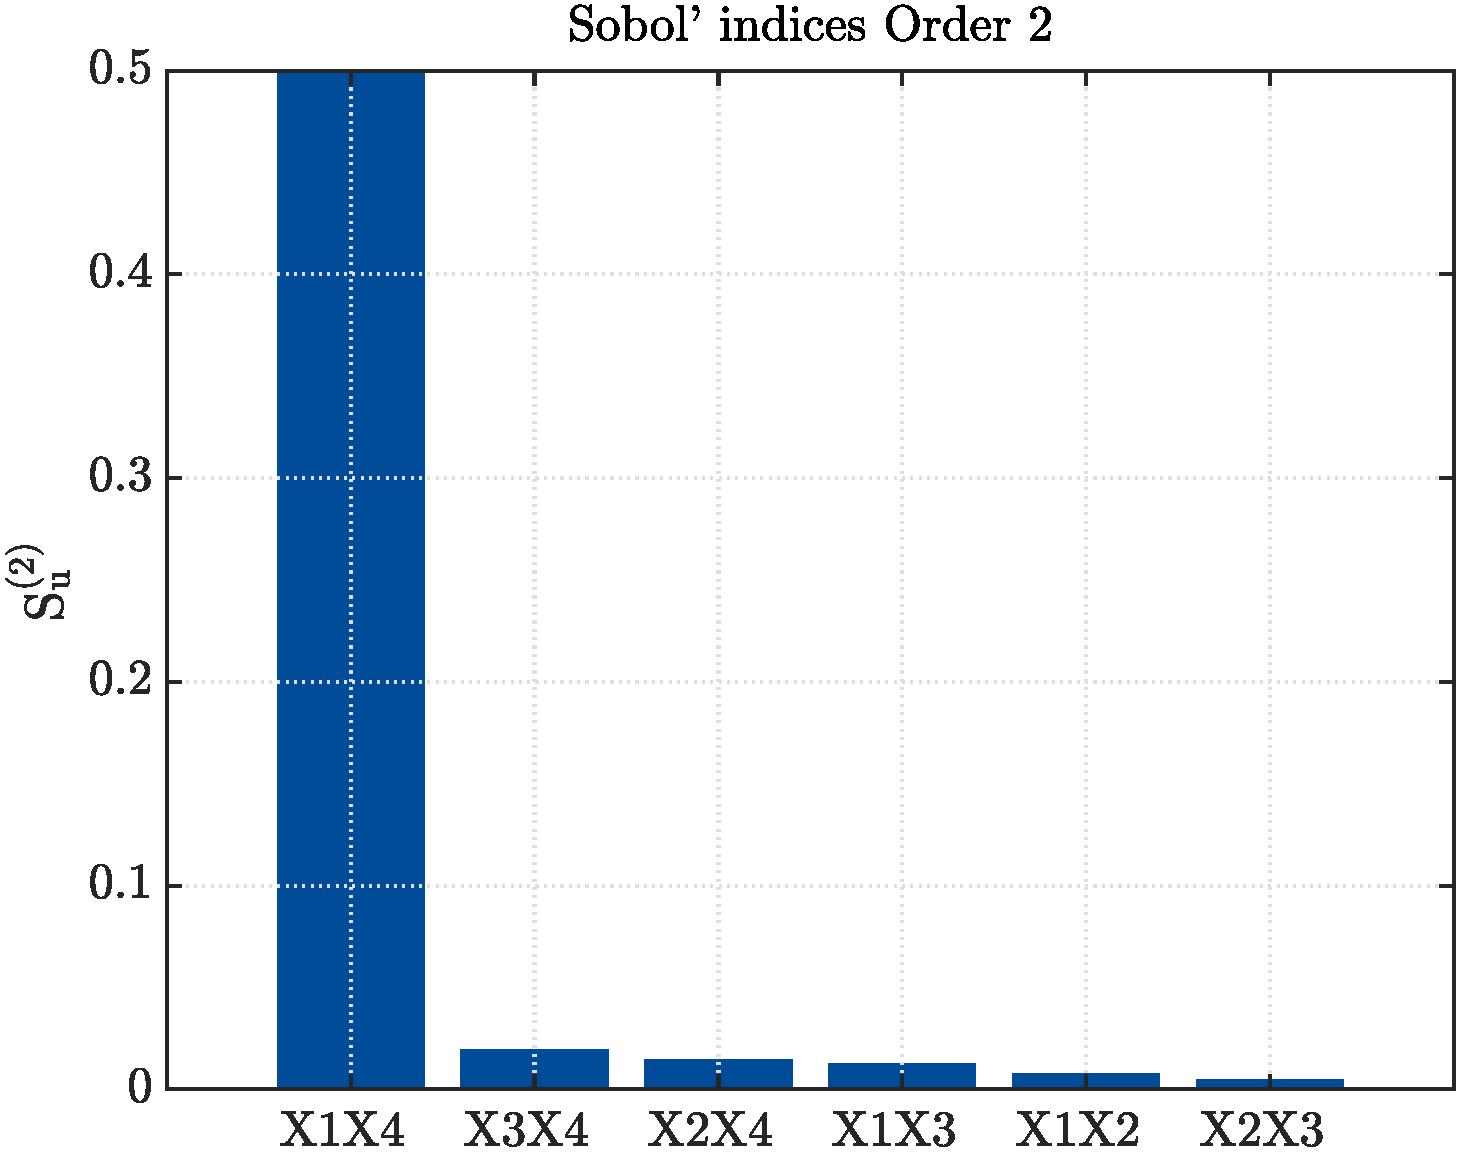
\includegraphics[width=\textwidth]{figures/second_type1.pdf}
	\caption{Second order.\label{fig:second_type1}}
	\end{subfigure}
	\caption{Sobol' indices for type 1.\label{fig:type1}}
\end{figure}

Classical analysis with type 2 access is shown in figure \ref{fig:type2}. In this case there are 3 input uncertainties, so $N=8M$ samples are necessary for total, first, and second order indices. One can note that 

\begin{figure}[hbtp]
\centering
	\begin{subfigure}[b]{.49\textwidth}
	\centering
	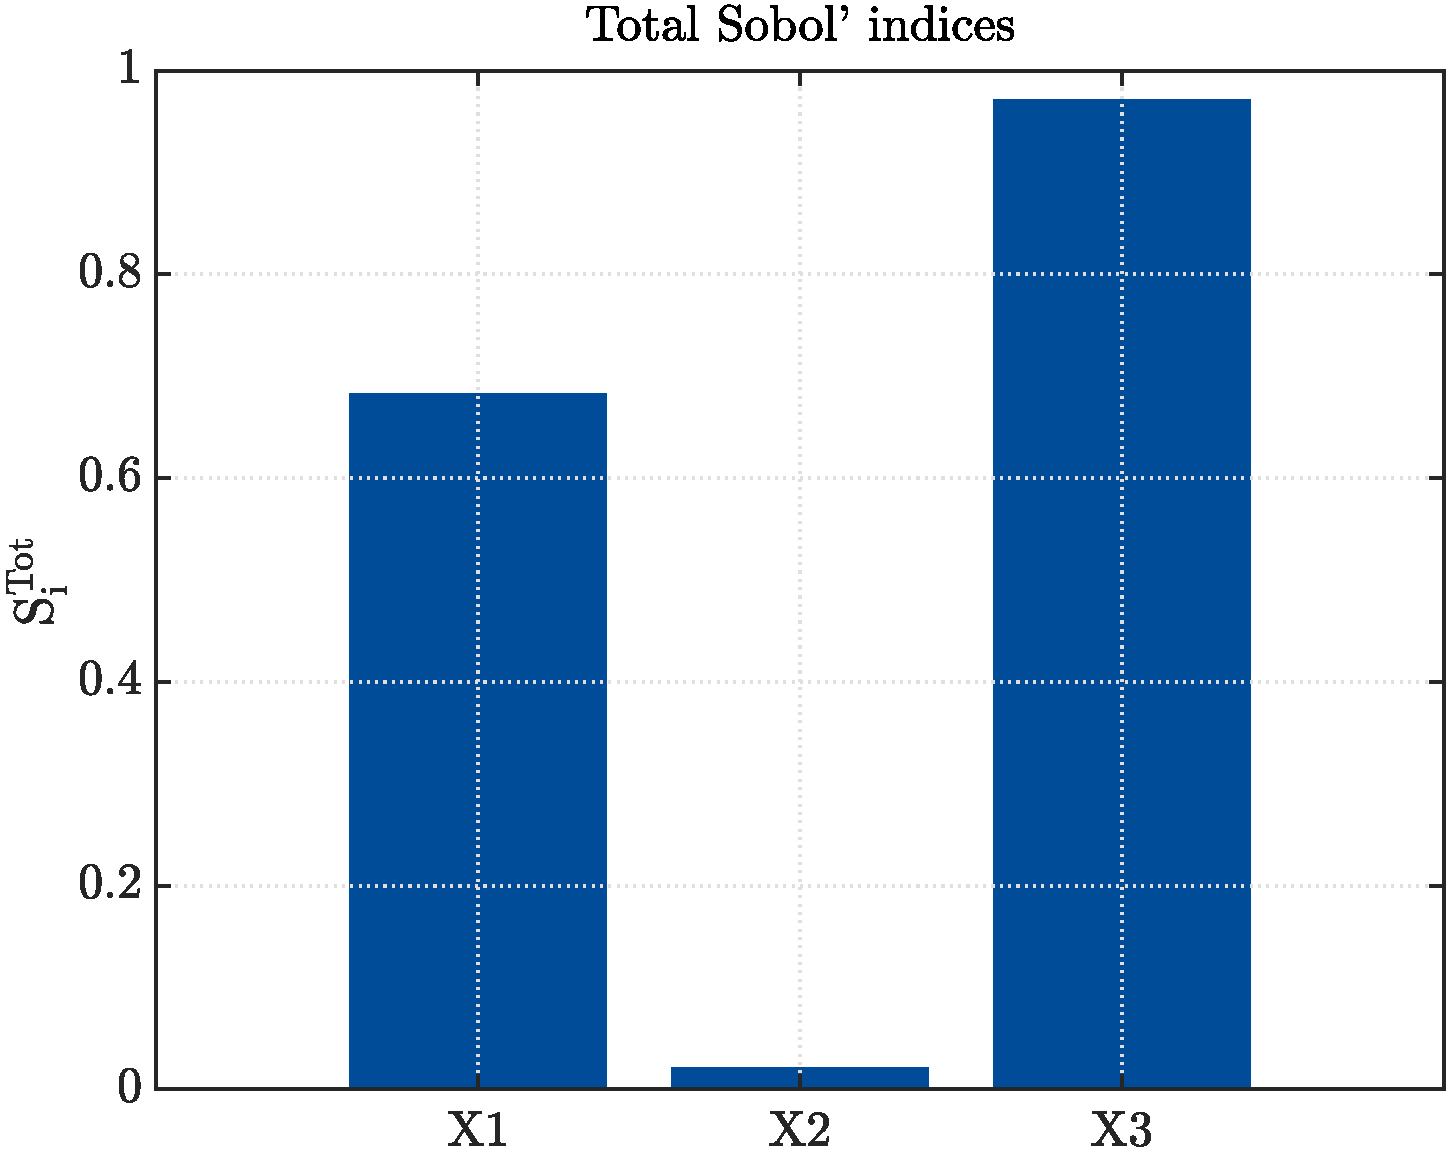
\includegraphics[width=\textwidth]{figures/total_type2.pdf}
	\caption{Total index.\label{fig:total_type2}}
	\end{subfigure}
	\hfill
	\begin{subfigure}[b]{.49\textwidth}
	\centering
	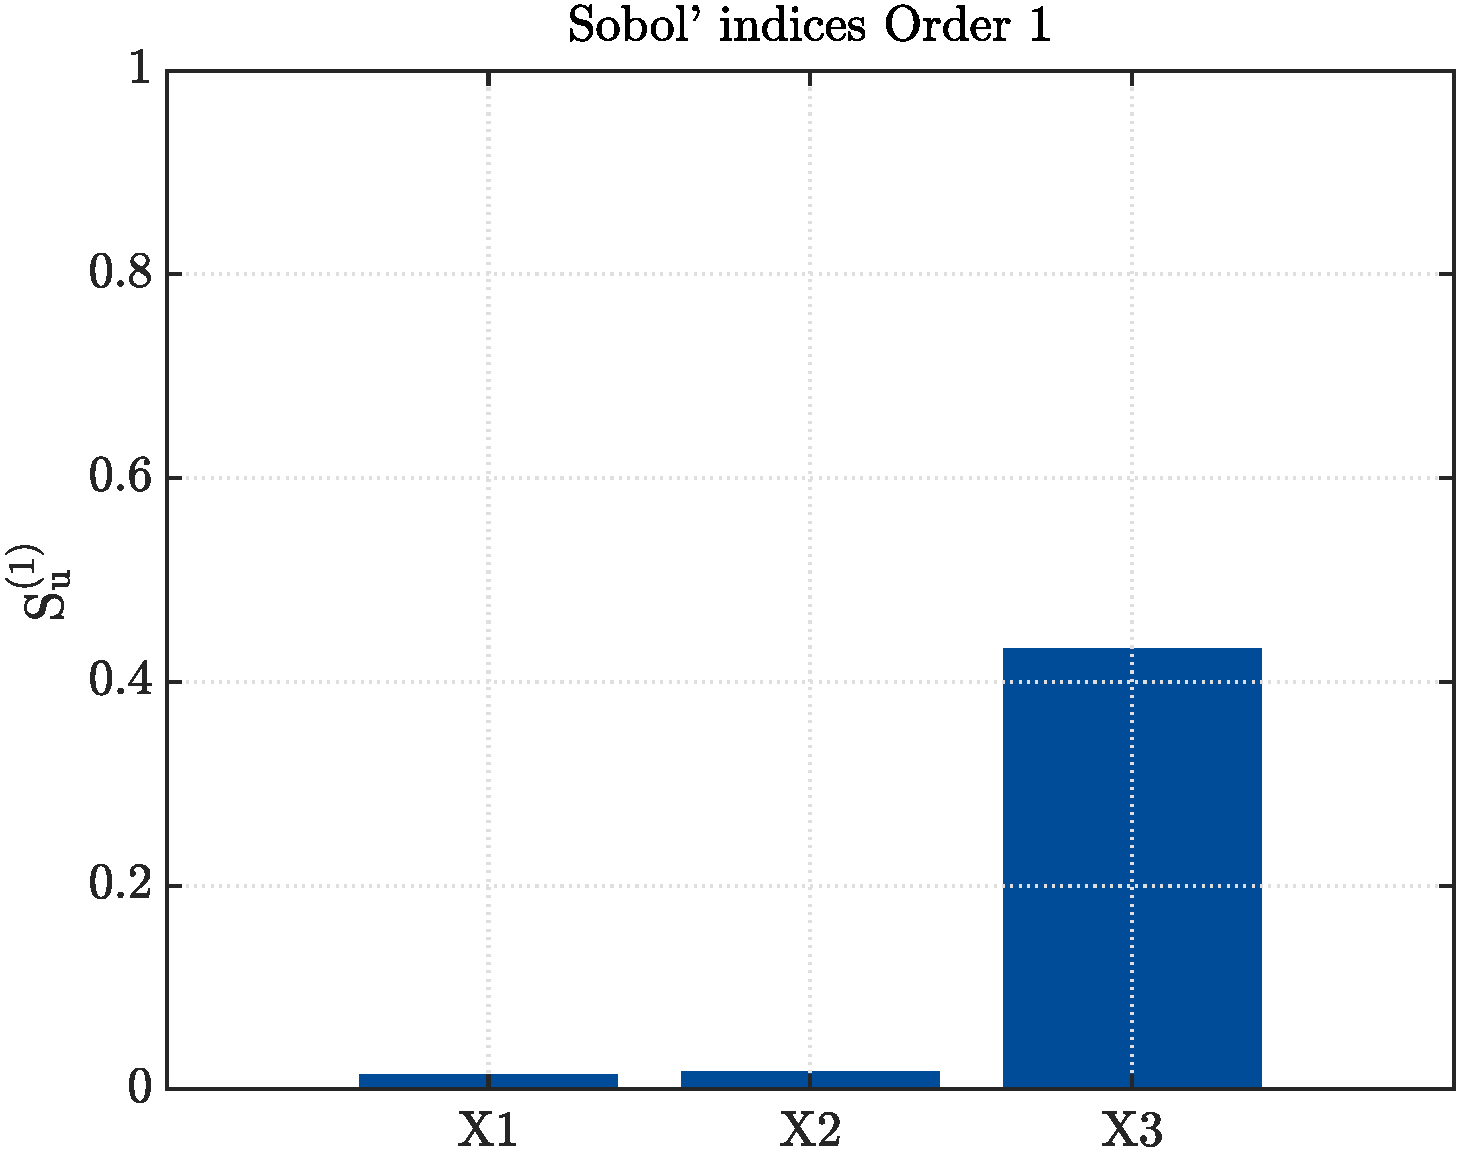
\includegraphics[width=\textwidth]{figures/first_type2.pdf}
	\caption{First order.\label{fig:first_type2}}
	\end{subfigure}\\
	\begin{subfigure}[b]{.49\textwidth}
	\centering
	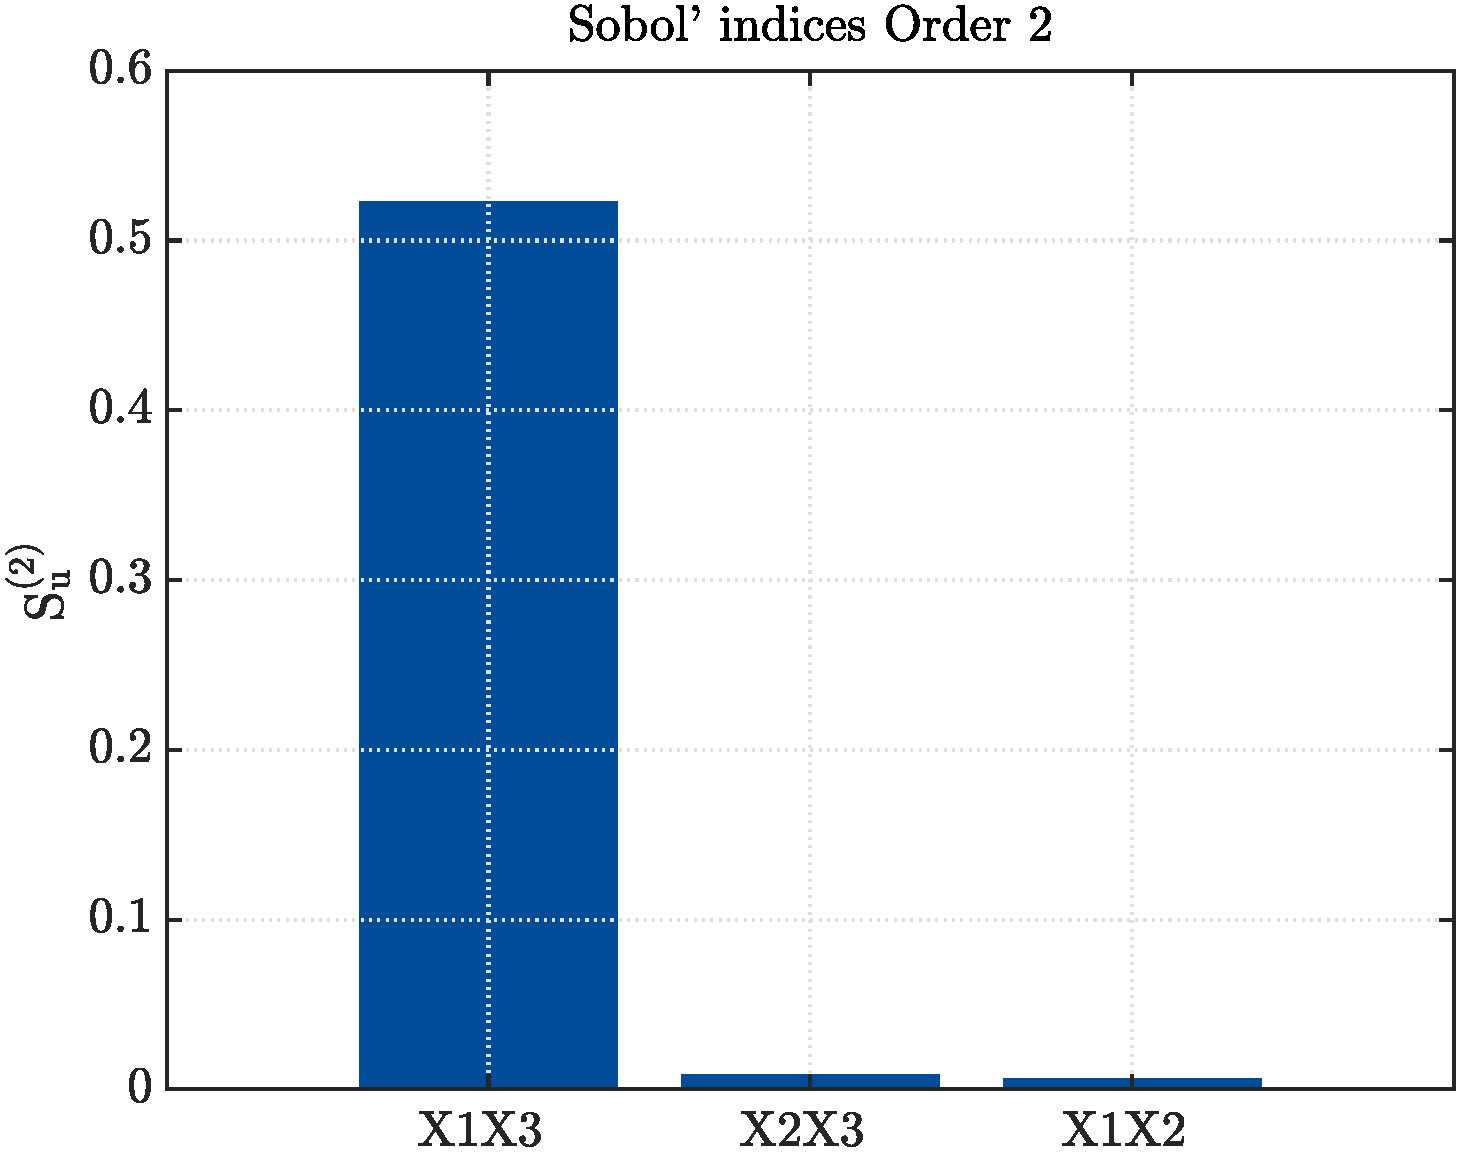
\includegraphics[width=\textwidth]{figures/second_type2.pdf}
	\caption{Second order.\label{fig:second_type2}}
	\end{subfigure}
	\caption{Sobol' indices for type 2.\label{fig:type2}}
\end{figure}

%\input{introduction.tex}

%\input{governing_equations.tex}
%
%\input{discretization.tex}
%
%\input{results.tex}
%
%\input{conclusions.tex}

%\section*{CRediT}
%\textbf{Benjamin Sanderse}: Conceptualization, Methodology, Software, Writing - Original Draft; \textbf{Jurriaan Buist}: Writing - Review \& Editing; \textbf{Ruud Henkes}: Resources,  Writing - Review \& Editing.

\FloatBarrier
%
%\appendix % Reset the chapter name and the chapter counting.
%
%\input{appendix.tex}


%%%%%%%%%%%%%%%%%%      References     %%%%%%%%%%%%%%%%%%
%\section*{\refname}
\section{References}
\bibliography{../../../../../../latex_documents/library}      % for an exte%rnal bibliography file
\bibliographystyle{abbrv}


\end{document}
